\chapter{Parallelization using Pipelining Technique}
\label{chap:pipeline}

The conventional 0/1-KPDP lends itself to a very straight-forward parallelization, because any element of a certain row of the dense table can be calculated independently of other elements of the same row, given the previous row. On the other hand, to calculate a row of the sparse table in SKPDP we use a process called \textit{Merge-Kill} which is inherently sequential.

The idea of using the pipelining technique stems from the understanding that the whole row of sparse table does not have to be calculated before starting the calculation of the next row. So, as a row of the sparse table is being computed, the values can be used immediately for calculating the next row. This way each thread is responsible for calculating one row of the sparse table and each thread acts as a consumer of the values produced by the previous thread. In hardware this can be implemented as streaming input to processing elements --REFERENCE--, but in software synchronization between threads is costly. So to minimize synchronization cost between threads the data between two consecutive threads can be shared in blocks instead of one data-point at a time. The block size is a very important parameter to be tuned in this algorithm, because too large of block size hinders parallelism and too small of a block size introduces more synchronization cost between threads.

Note that using this technique we only completely write out every $p$-th row of sparse table into memory. So, the the $(p-1)$-th thread is responsible for maintaining a whole row, where the threads 0 to $p-2$ maintain a local buffer of size $w_i$. 


\begin{figure}[htbp]
\centerline{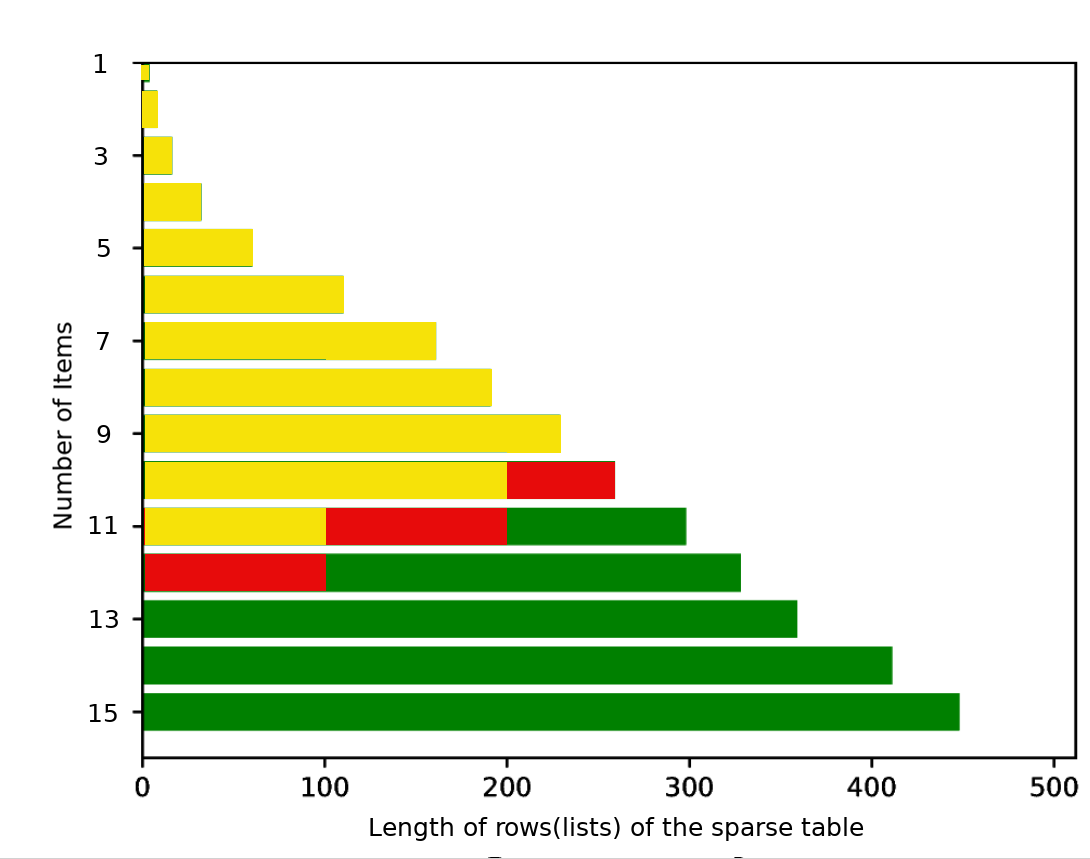
\includegraphics[width=1\columnwidth]{images/pipelining.png}}
\caption{Pipelining (coarse-grained) parallelism of KSPDP }
\label{fig:pipeline}
\end{figure}

Figure \ref{fig:pipeline} represents the idea of pipelining in the context of SKPDP. Let's take a small knapsack problem instance with $n=15$ and $C=512$ for demonstration purposes. The horizontal bars represents the size of each row of the sparse table. The yellow colored parts are already calculated; the red blocks are being calculated in parallel and the green parts are yet to be calculated.

\paragraph{Overhead Analysis} Most of the overhead of the computation comes from block synchronization and additional memory reads and writes of our current implementation which still requires some optimization. The space-complexity of this algorithm is $O(2nC + w_{max}p)$ because of the $p$ thread have to maintain a buffer of $w_i$.